\chapter{Paper I:\@
  Mechanism of Pd(II)-mediated\linebreak uncaging reactions % chktex 36
  of propargylic substrates
 }%
\label{ch:paper1}

\citetext{Coelho2019}

An application to metallocatalysis~\cite{Coelho2019}.
A computational-experimental collaboration.



HOW IS THE RESEARCH DESIGNED?\@

WHY IT IS DESIGNED THIS WAY?\@




WHAT DOES THE LITERATURE SAY ABOUT THIS?\@

IS THE LITERATURE WELL STABLISHED?\@
IS IT DIVIDED?\@

HOW DOES THE RESEARCH FIT THE BIGGER PICTURE?\@

HOW DOES THE RESEARCH CONTRIBUTE SOMETHING ORIGINAL?\@

HOW DOES THE METHODOLOGY OF PREVIOUS STUDIES HELP YOU DEVELOP YOUR OWN?\@







WHY IS THIS WORTH INVESTIGATING?\@
HOW IMPORTANT IS THIS?\@
HOW IS THIS ORIGINAL?\@

WHAT WERE MY RESEARCH AIMS?\@

WHAT IS THE SCOPE OF MY STUDY?\@
WHAT I COVERED AND DIDN'T COVER?\@

WHICH METHODS WERE USED?\@




\section{Background and motivation}

PRESENTATION OF THE WORK.\@

DESCRIPTION OF THE WORK.\@

OBJECTIVES OF THE WORK.\@

INTERPRETATION AND MEANING OF THE WORK.\@

MAIN FINDINGS.\@

RESULTS IN RELATION TO THE RESEARCH QUESTIONS.\@

\section{Paper}

The publication can be read in full next.

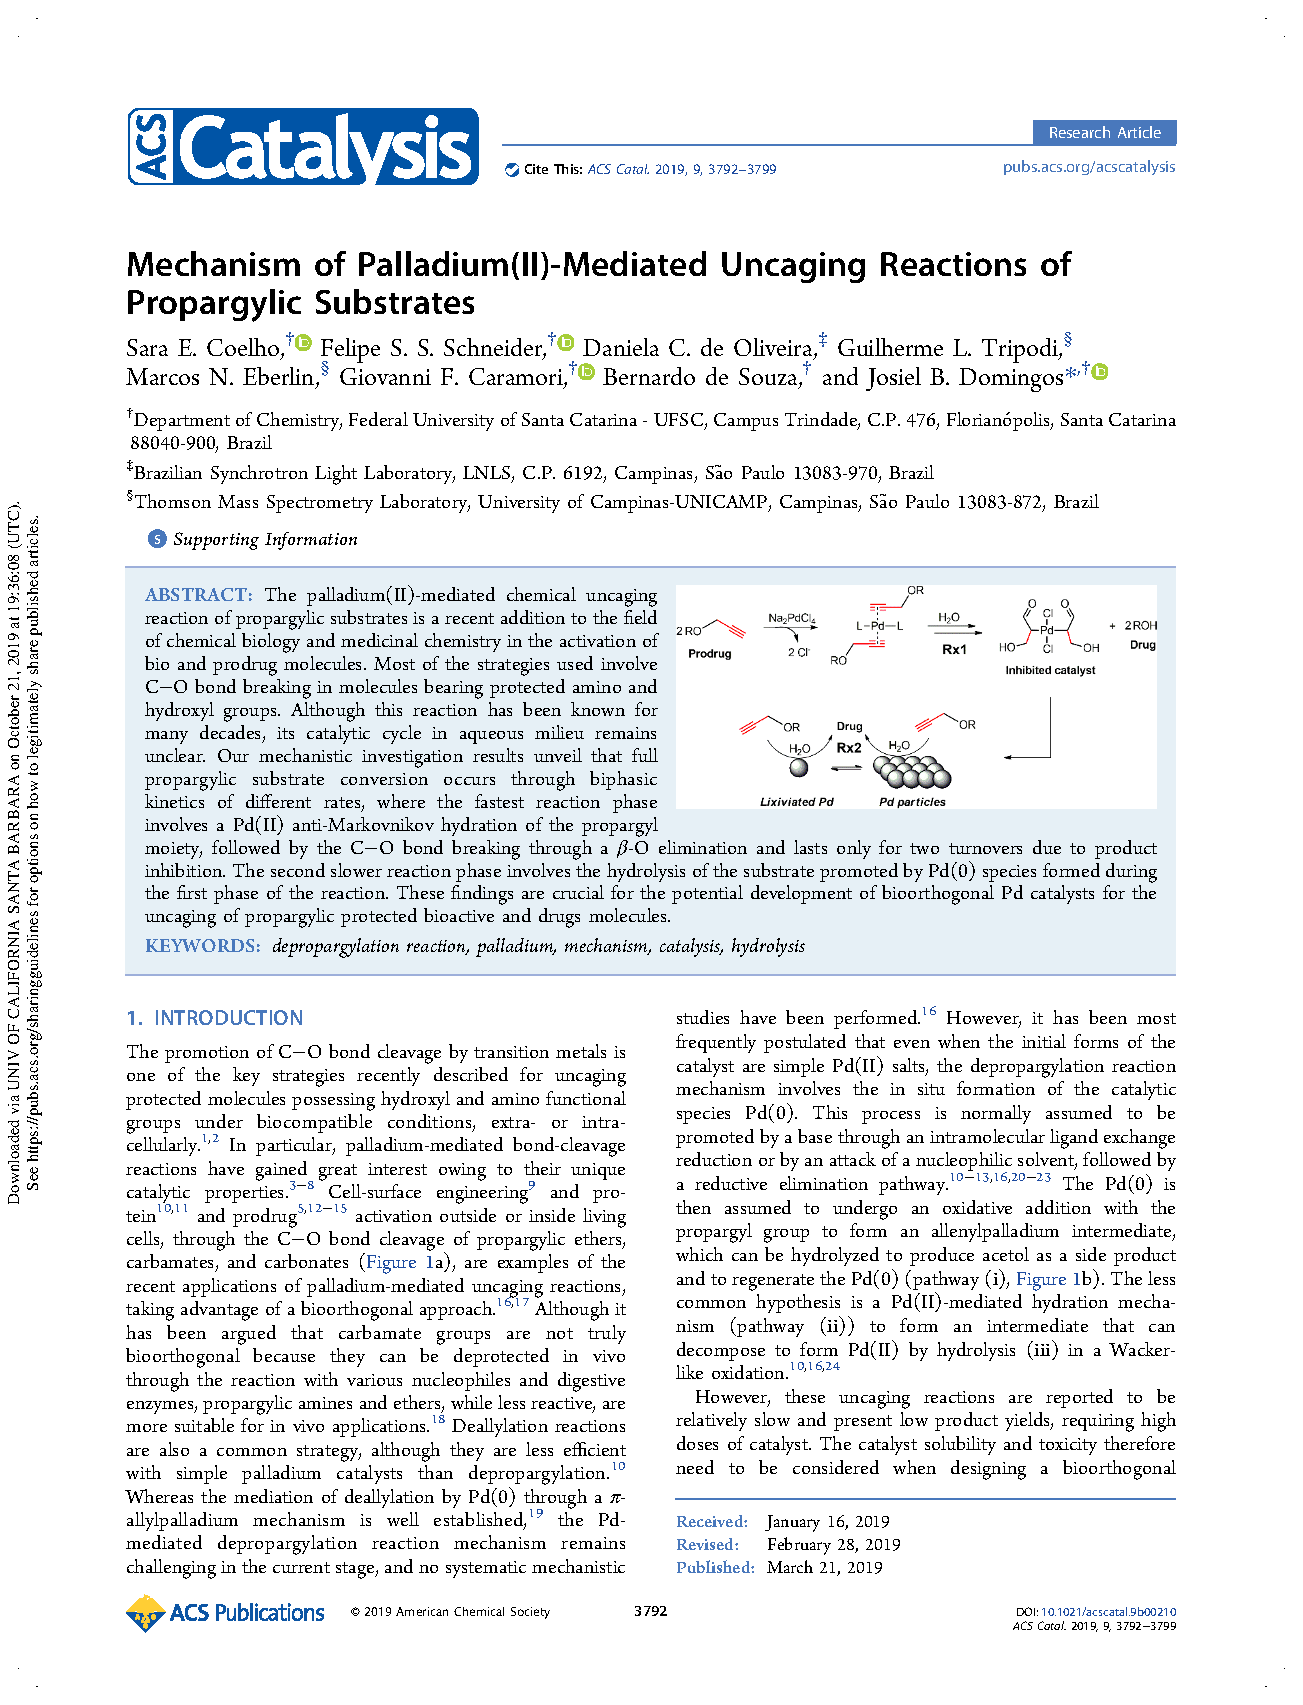
\includepdf[pages=-]{pubs/coelho2019-paper1.pdf}
